\documentclass[12pt]{article}
 
\usepackage[margin=1in]{geometry} 
\usepackage{amsmath,amsthm,amssymb}
\usepackage{graphicx}
\usepackage{bbold}
\usepackage{multirow}

\newcommand{\N}{\mathbb{N}}
\newcommand{\Z}{\mathbb{Z}}
\newcommand{\E}{\mathbb{E}}
\newcommand{\Prob}{\text{Prob}}


\begin{document}
\title{\large \textbf{The TANK Model with CBDC, Bank and Dollarization}}
\date{}
\maketitle
\section{Model without Dollarization}
This model is an extension of the TANK model in a small open economy, with CBDC and a monopolistic competitive bank sector. Deposit, cash and CBDC provide liquidity service and decrease the transaction cost. Banks take deposits from unconstrained households and invest in intermediate firms; constrained households do not have access to bank services and can only hold cash or CBDC. 

\subsection{Households}
The consumption bundle is defined as follows:
\begin{align*}
c_t = [\gamma^{\frac{1}{\eta}}c_{Ht}^{\frac{\eta-1}{\eta}}+(1-\gamma)^{\frac{1}{\eta}}c_{Ft}^{\frac{\eta-1}{\eta}}]^{\frac{\eta}{\eta-1}}, 
\end{align*}
where $c_{Ht}$ and $c_{Ft}$ denote consumption of domestic and foreign final good respectively. $\gamma$ is the home bias. The representative household decides how to allocate her consumption expenditure between domestic and foreign goods.

By solving the static optimization problem, the optimal consumption of domestic and foreign final goods can be solved as 
\begin{align*}
c_{Ht} &= \gamma(\frac{P_{Ht}}{p_t})^{-\eta}, \\
c_{Ft} &= (1-\gamma)(\frac{P_{Ft}}{p_t})^{-\eta}, 
\end{align*}
where $p_t$ is the domestic CPI, i.e., the price of one unit of consumption: 
\begin{align*}
p_t = [\gamma P_{Ht}^{1-\eta}+(1-\gamma)P_{Ft}^{1-\eta}]^{\frac{1}{1-\eta}}.
\end{align*}
In a small open economy, the price of the foreign good coincides with the foreign CPI $p_t^*$, adjusted by the nominal exchange rate $e_t$:
\begin{align*}
P_{Ft} = e_tp_t^*
\end{align*}
The real exchange rate is defined as the ratio of the foreign and domestic price levels, where the foreign price level is converted into domestic currency units via the nominal exchange rate: 
\begin{align*}
\xi_t = e_t \frac{p_t^*}{p_t}
\end{align*}
Define $p_{Ht} = P_{Ht}/p_t$ and  $p_{Ft} = P_{Ft}/p_t$ as the price of domestic and foreign goods in terms of the domestic CPI, then the real exchange rate can be written as: 
\begin{align*}
\xi_t = p_{Ft}, 
\end{align*}
and the terms of trade, i.e., the ratio between the price imports and the price exports can be written as 
\begin{align*}
tot_t = \frac{P_{Ft}}{P_{Ht}} = \frac{\xi_t}{p_{Ht}}
\end{align*}

\subsubsection*{Unconstrained HH ($1-\lambda$)} 
Unconstrained households with measure $1-\lambda$ have access to the bank service. Each period, they choose their consumption $c_{1t}$ and labor supply $h_{1t}$ and receive labor income $\omega_t$. Unconstrained households pay consumption tax at the rate $\tau_c$. They also receive a lump-sum transfer from the government $t_{1t}$ and profit of intermediate firms and banks $\Gamma_{1t}$.

Unconstrained households face liquidity constraints. I follow Schmitt-Groh{\'e} and Uribe (2007) and assume that the transaction cost of consumption $s_{1t}$ is determined by the Transaction Cost Function:
\begin{align*}
s_{1t} = z_tA_1\frac{c_{1t}}{l_{1t}}+B_1\frac{l_{1t}}{c_{1t}}-2\sqrt{A_1B_1},
\end{align*}
where the ratio between consumption and liquidity $c_{1t}/l_{1t}$ represents the money velocity, the transaction cost is increasing in the velocity as long as the following condition is satisfied:  
\begin{align*}
\frac{c_{1t}}{l_{1t}}>\sqrt{\frac{B_1}{z_tA_1}}.
\end{align*} 

Unconstrained households get liquidity services from commercial banks. There is a continuum measure of monopolistic competitive banks index by $j \in [0,1]$. Bank deposits are substitutes with the elasticity of substitution $\epsilon_b > 1$. The total liquidity for unconstrained households can be written as: 
\begin{align}
\label{l1t}
l_{1t} = \int_0^1({d_{1t}(j)}^{\frac{\epsilon_b-1}{\epsilon_b}}dj)^{\frac{\epsilon_b}{\epsilon_b-1}} 
\end{align}

The return to deposit $r_t^d(j)$ is determined by the bank sector optimization problem. Unconstrained households also hold one-period government bond $b_{1Ht}$ and foreign bond $b_{1Ft}$, with $r_t$ and $r_t^*$ being the nominal interest rate of bonds. 

Domestic households pay a quadratic adjustment cost when they change their financial position (foreign bond and foreign currency) with the rest of the world: this assumption ensures the existence of a determinate steady state and a stationary solution. (Schmitt-Groh{\'e} and Uribe, 2003)

The unconstrained households' problem can be defined as (all variables are in real terms):
\begin{align*}
\max_{c_{1t}, h_{1t},s_{1t},l_{1t},d_{1t}(j),b_{1Ht},b_{1Ft}} E_0 \sum_0^{\infty}\beta^t (\frac{c_{1t}^{1-\sigma}}{1-\sigma}-\chi\frac{h_{1t}^{1+\phi}}{1+\phi}),
\end{align*}
subject to the budget and liquidity constraints:
\begin{align*} 
&(1+s_{1t}+\tau_c)c_{1t}+\int_0^1(d_{1t}(j)-\frac{r_{t-1}^d(j)}{\pi_t}d_{1t-1}(j))dj +(b_{1Ht}-\frac{r_{t-1}}{\pi_t}b_{1Ht-1})+\xi_t(b_{1Ft}-r^*_{t-1}b_{1Ft-1}) \\
&\leq w_th_{1t}+t_{1t}+\Gamma_{1t}-\frac{\kappa_B}{2}\xi_t((1-\lambda)b_{1Ft}-\bar{b}_F)^2 \quad (\lambda_{1t}) \\
&l_{1t} = \int_0^1({d_{1t}(j)}^{\frac{\epsilon_b-1}{\epsilon_b}}dj)^{\frac{\epsilon_b}{\epsilon_b-1}} \quad (\tau_{1t}\lambda_{1t}) \\
&s_{1t} = z_tA_1\frac{c_{1t}}{l_{1t}}+B_1\frac{l_{1t}}{c_{1t}}-2\sqrt{A_1B_1}  \quad (\mu_{1t}\lambda_{1t})
\end{align*}
Taking first order conditions with respect to $c_{1t}, h_{1t}, s_{1t}, l_{1t}, d_{1t}(j), b_{1Ht}, b_{1Ft}$: 
\begin{align}
\label{c1}
c_{1t}: \quad &c_{1t}^{-\sigma}-\lambda_{1t}(1+s_{1t}+\tau_c)+\tau_{1t}\lambda_{1t}(z_tA_1\frac{1}{l_{1t}}-B_1\frac{l_{1t}}{c_{1t}^2}) = 0, \\
\label{h1}
h_{1t}: \quad &-\chi h_{1t}^{\phi}+\lambda_{1t}\omega_t  = 0, \\
\label{s1}
s_{1t}: \quad &-\lambda_{1t}c_{1t}-\tau_{1t}\lambda_{1t} = 0, \\
\label{l1}
l_{1t}: \quad &\tau_{1t}\lambda_{1t}(-z_tA_1\frac{c_{1t}}{l_{1t}^2}+B_1\frac{1}{c_{1t}})-\mu_{1t}\lambda_{1t} = 0, \\
\label{d1j}
d_{1t}(j): \quad &-\lambda_{1t}+\beta E_t\lambda_{1t+1}\frac{r_{t}^d(j)}{\pi_{t+1}}+\mu_{1t}\lambda_{1t}(\frac{l_{1t}}{d_{1t}(j)})^{\frac{1}{\epsilon_b}} = 0, \\
\label{b1H}
b_{1Ht}: \quad &-\lambda_{1t}+\beta E_t\lambda_{1t+1}\frac{r_t}{\pi_{t+1}} = 0, \\
\label{b1F}
b_{1Ft}: \quad &-\lambda_{1t}+\beta E_t\lambda_{1t+1}\frac{\xi_{t+1}}{\xi_t}t_t^*-\lambda_{1t}\kappa_B(1-\lambda)((1-\lambda)b_{1Ft}-\bar{b}_F) = 0,
\end{align}
Define the transaction wedge as:
\begin{align}
\label{tau1c}
\tau_{1t}^c = z_tA_1\frac{c_{1t}}{l_{1t}}-B_1\frac{l_{1t}}{c_{1t}}.
\end{align}
Plug (\ref{tau1c}) into first order condition (\ref{c1}) and (\ref{h1}), the intertemporal and intratemporal euler equation can be written as: 
\begin{align*}
c_{1t}^{-\sigma} &= \lambda_{1t}(1+s_{1t}+\tau_c+\tau_{1t}^c) \\
\lambda_{1t}(1-\frac{c_{1t}}{l_{1t}}\tau_{1t}^c(\frac{l_{1t}}{d_{1t}(j)})^{\frac{1}{\epsilon_b}}) &= \beta \E_t\lambda_{1t+1}\frac{r_{t}^d(j)}{\pi_{t+1}} \\
\chi h_{1t}^{\phi} &= \lambda_{1t}\omega_t 
\end{align*}
Combine equation (\ref{l1}), (\ref{d1j}) and (\ref{b1H}), then plug in (\ref{tau1c}), we can get: 
\begin{align*}
\beta E_t\lambda_{1t+1}\frac{r_{Ht}^d(j)}{\pi_{t+1}} = \beta E_t\lambda_{1t+1}\frac{r_t}{\pi_{t+1}}(1-\frac{c_{1t}}{l_{1t}}\tau_{1t}^c(\frac{d_{1Ht}}{d_{1Ht}(j)})^{\frac{1}{\epsilon_b}}). 
\end{align*}
Then plug the equation above to equation (\ref{l1t}), the demand function for $d_{1t}(j)$ can be derived as:
\begin{align}
d_{1t}(j) = \Biggl(\frac{(r_t-r_t^d(j))^{-\epsilon_b}}{\big(\int_0^1(r_t-r_t^d(j))^{1-\epsilon_b}dj\big)^{-\frac{\epsilon_b}{1-\epsilon_b}}}\Biggl)d_{1t}
\end{align}

\subsubsection*{Constrained HH ($\lambda$)}
The constrained households with measure $\lambda$ don't have access to bank services, so they don't have access to bank deposits or government bonds. Each period, they choose their consumption $c_{2t}$ and labor supply $h_{2t}$ and receive labor income $\omega_t$. Unconstrained households pay consumption tax at rate $\tau_c$, but only when the payment is made by CBDC. They also receive a lump-sum transfer from the government $t_{2t}$. 

Constrained households face the same liquidity constraints as unconstrained households. They can only get liquidity service by holding cash ($m_{2t}$) or CBDC ($CBDC_{2t}$). Cash users are facing an additional cost $\delta_m$ since cash is at risk of being stolen and subject to an adjustment cost. CBDC is a safer and more convenient liquid asset, so it's free of risk and adjustment costs. Cash and CBDC are substitutes with the elasticity of substitution $\epsilon_m>1$. The total liquidity for constrained households can be written as: 
\begin{align*}
l_{2t} = ((m_{2t})^{\frac{\epsilon_m-1}{\epsilon_m}}+(CBDC_{2t})^{\frac{\epsilon_m-1}{\epsilon_m}})^{\frac{\epsilon_m}{\epsilon_m-1}}
\end{align*}

The constrained households' problem can be defined as (all variables are in real terms):
\begin{align*}
\max_{c_{2t}, h_{2t},l_{2t},s_{2t},m_{2t},CBDC_{2t}} E_0 \sum_0^{\infty}\beta^t (\frac{c_{2t}^{1-\sigma}}{1-\sigma}-\chi\frac{h_{2t}^{1+\phi}}{1+\phi})
\end{align*}
subject to the budget and liquidity constraints:
\begin{align*} 
\text{s.t.} \quad & (1+s_{2t}+\tau_c\frac{CBDC_{2t}}{l_{2t}})c_{2t}+(m_{2t}-\frac{1-\delta_m}{\pi_t}m_{2t-1})+(CBDC_{2t}-\frac{1}{\pi_t}CBDC_{2t-1}) \\
&\leq w_th_{2t}+t_{2t}\\
&l_{2t} = ((m_{2t})^{\frac{\epsilon_m-1}{\epsilon_m}}+(CBDC_{2t})^{\frac{\epsilon_m-1}{\epsilon_m}})^{\frac{\epsilon_m}{\epsilon_m-1}}  \quad (\tau_{2t}\lambda_{2t})\\
& s_{2t} = z_tA_2\frac{c_{2t}}{l_{2t}}+B_2\frac{l_{2t}}{c_{2t}}-2\sqrt{A_2B_2} \quad (\mu_{2t}\lambda_{2t})
\end{align*}
Taking first order conditions with respect to $c_{2t}, h_{2t}, s_{2t}, l_{2t}, m_{2t}, CBDC_{2t}$: 
\begin{align}
\label{c2}
c_{2t}: \quad &c_{2t}^{-\sigma}-\lambda_{2t}(1+s_{2t}+\tau_c\frac{CBDC_{2t}}{l_{2t}})+\tau_{2t}\lambda_{2t}(z_tA_2\frac{1}{l_{2t}}-B_2\frac{l_{2t}}{c_{2t}^2}) = 0, \\
\label{h2}
h_{2t}: \quad &-\chi h_{2t}^{\phi}+\lambda_{2t}\omega_t  = 0, \\
\label{s2}
s_{2t}: \quad &-\lambda_{2t}c_{2t}-\tau_{2t}\lambda_{2t} = 0, \\
\label{l2}
l_{2t}: \quad &\lambda_{2t}\tau_c\frac{CBDC_{2t}}{l_{2t}^2}c_{2t}+\tau_{2t}\lambda_{2t}(-z_tA_2\frac{c_{2t}}{l_{2t}^2}+B_2\frac{1}{c_{2t}})-\mu_{2t}\lambda_{2t} = 0, \\
\label{m2}
m_{2t}: \quad &-\lambda_{2t}+\beta E_t\lambda_{2t+1}\frac{1-\delta_m}{\pi_{t+1}}+\mu_{2t} \lambda_{2t}(\frac{l_{2t}}{m_{2t}})^{\frac{1}{\epsilon_m}}= 0, \\
\label{CBDC2}
CBDC_{2t}: \quad &-\lambda_{2t}(1+\tau_c\frac{c_{2t}}{l_{2t}})+\beta E_t\lambda_{2t+1}\frac{1}{\pi_{t+1}}+\mu_{2t} \lambda_{2t}(\frac{l_{2t}}{CBDC_{2t}})^{\frac{1}{\epsilon_m}}= 0.
\end{align}
Similar to the unconstrained households, we can define the transaction wedge as:
\begin{align}
\label{tau2c}
\tau_{2t}^c = z_tA_2\frac{c_{2t}}{l_{2t}}-B_2\frac{l_{2t}}{c_{2t}}.
\end{align}
Plug (\ref{tau2c}) into first order condition (\ref{c2}) and  (\ref{h2}), combine with equation (\ref{m2}), the intertemporal and intratemporal euler equation can be written as: 
\begin{align*}
c_{2t}^{-\sigma} &= \lambda_{2t}(1+s_{2t}+\tau_{2t}^c+\tau_c\frac{CBDC_{2t}}{l_{2t}}) \\
\lambda_{2t}(1-\frac{c_{2t}}{l_{2t}}(\tau_{2t}^c+\tau_c\frac{CBDC_{2t}}{l_{2t}})(\frac{l_{2t}}{m_{2t}})^{\frac{1}{\epsilon_m}}) &= \beta E_t \lambda_{2t+1} \frac{1-\delta_m}{\pi_{t+1}}, \\
\chi h_{1t}^{\phi} &= \lambda_{1t}\omega_t 
\end{align*}
The no-arbitrage condition for cash and CBDC can be derived from equations (\ref{m2}) and (\ref{CBDC2}).

\subsection{Bank}
There is a continuum measure of monopolistic competitive banks $j \in [0,1]$. They take deposits from unconstrained households $d_{t}(j)$ and invest in intermediate firms $i_t(j)$ and accumulate capital stock $k_t(j)$. The deposit demand functions are solved from the household problem above. 
\begin{align*}
d_{t}(j) = \Biggl(\frac{(r_t-r_t^d(j))^{-\epsilon_b}}{\big(\int_0^1(r_t-r_t^d(j))^{1-\epsilon_b}dj\big)^{-\frac{\epsilon_b}{1-\epsilon_b}}}\Biggl)d_{t} 
\end{align*}

Banks are owned by unconstrained households, so bankers maximize its expected pre-dividend profits: 
\begin{align*}
 &\max_{r_t^d(j),i_t(j),k_t(j)}E_0 \sum_0^{\infty}\beta^t\frac{\lambda_{1t}}{\lambda_{10}}(r_t^kk_{t-1}(j)-i_t(j)+(d_{t}(j)-\frac{r_{t-1}^d(j)}{\pi_t}d_{t-1}(j)),
 \end{align*}
subject to the law of motion of capital and balance sheet constraint: 
 \begin{align*}
  \quad & k_t(j) = (1-\delta)k_{t-1}(j)+(1-\frac{\kappa_I}{2}(\frac{i_t(j)}{i_{t-1}(j)}-1))i_t(j), \\
& k_t(j) = d_{t}(j).
\end{align*}

The equilibrium is symmetric; then the first-order conditions give the supply for new investment 
\begin{align*}
\lambda_{1t} = q_t\lambda_{1t}(1-\frac{\kappa_I}{2}(\frac{i_t}{i_{t-1}}-1)^2-\kappa_I(\frac{i_t}{i_{t-1}}-1)\frac{i_t}{i_{t-1}})+ \beta\E_tq_{t+1}\lambda_{1t+1}\kappa_I(\frac{i_{t+1}}{i_t}-1)^2(\frac{i_{t+1}}{i_t})^2,
\end{align*}
and optimal deposit rate is chosen by the bank:  
\begin{align*}
{r_{t}^d}^* &= \frac{\epsilon_b}{\epsilon_b-1}\frac{\beta E_t \lambda_{1t+1}(r_{t+1}^k+(1-\delta)q_{t+1})-(q_t-1)\lambda_{1t}}{\beta E_t (\lambda_{1t+1}/\pi_{t+1})}-\frac{1}{\epsilon_b-1}r_t.
\end{align*}
When $\epsilon_b \to \infty$, then banks are perfectly competitive, then the deposit rate chosen by the bank becomes the net return to capital: 
\begin{align*}
{r_{t}^d}^* &= \frac{\beta E_t \lambda_{1t+1}(r_{t+1}^k+(1-\delta)q_{t+1})-(q_t-1)\lambda_{1t}}{\beta E_t (\lambda_{1t+1}/\pi_{t+1})}.
\end{align*}

\subsection{Firm}
The firm problem is standard. The representative final-good firm uses the following CES aggregator to produce the domestic final good, and the intermediate firms produce differentiated domestic input. 

\subsubsection*{Final}
The representative final-good firm uses the following CES aggregator to produce the domestic final good $y_{Ht}$:
\begin{align*}
y_{Ht} = (\int_0^1 y_{Ht}(i)^{\frac{\epsilon}{\epsilon-1}})^{\frac{\epsilon-1}{\epsilon}}
\end{align*}
where $y_{Ht}(i)$ is an intermediate input produced by the intermediate firm $i$, whose price is $P_{Ht}(i)$. The final good firm maximizes the profit: 
\begin{align*}
\max_{y_{Ht},y_{Ht}(i)}\quad P_{Ht}(\int_0^1 y_{Ht}(i)^{\frac{\epsilon}{\epsilon-1}})^{\frac{\epsilon-1}{\epsilon}}- \int_0^1 P_{Ht}(i)y_{Ht}(i)
\end{align*}
Then the first order conditions give the demand for intermediate goods: 
\begin{align*}
y_{Ht}(i) = y_{Ht}\Big(\frac{P_{Ht}(i)}{P_{Ht}}\Big)^{-\epsilon}
\end{align*}

\subsubsection*{Intermediate}
There is a continuum of firms indexed by $i$ producing a differentiated domestic input using the following Cobb-Douglas function:
\begin{align*}
y_{Ht}(i) = a_t(k_{t-1}(i))^{\alpha}(h_t(i))^{1-\alpha}
\end{align*}
where $a_t$ is the total factor productivity, which follows an autoregressive process: 
\begin{align*}
\log(a_t) = \rho_a\log(a_{t-1})+\nu_t^a, \quad  \nu_t^a \sim N(0,\sigma_a^2)
\end{align*}
Firms operate in monopolistic competition, so they set the price of their own good subject to the demand of final good firms. In addition, firms pay quadratic adjustment cost $AC_t(i)$ in nominal terms as in Rotemberg (1982), whenever they adjust prices with respect to the benchmark inflation rate $\bar{\pi}$:
\begin{align*}
AC_t(i) = \frac{\kappa_P}{2}\Big(\frac{P_{Ht}(i)}{P_{Ht-1}(i)}-\bar{\pi}\Big)^2P_{Ht}y_{Ht}
\end{align*}
The intermediate firm is owned by unconstrained households and maximizes the profit: 
\begin{align*}
\max_{P_{Ht}(i),y_{Ht}(i),k_{t-1}(i), h_t(i)} &E_0 \sum_0^{\infty}\beta^t\frac{\lambda_{1t}}{\lambda_{10}}(\frac{P_{Ht}(i)}{p_t}y_{Ht}(i)-w_th_t(i)-r_t^kk_{t-1}(i)-\frac{AC_t(i)}{p_t}),
\end{align*}
subject to the production and demand function: 
\begin{align*}
y_{Ht}(i) &= a_t(k_{t-1}(i))^{\alpha}(h_t(i))^{1-\alpha}, \\
y_{Ht}(i) &= y_{Ht}\Big(\frac{P_{Ht}(i)}{P_{Ht}}\Big)^{-\epsilon}.
\end{align*}

The equilibrium is symmetric, the equilibrium interest rate and wage can be solved as: 
\begin{align*}
r_t^k &= \alpha mc_t \frac{y_{Ht}}{k_{t-1}}, \\
\omega_t &= (1-\alpha) mc_t \frac{y_{Ht}}{h_t}.
\end{align*}
The marginal cost $mc_t$ is defined by rearranging the price condition: 
\begin{align*}
\frac{\epsilon}{\kappa_P}(\frac{mc_t}{p_{Ht}}-\frac{\epsilon-1}{\epsilon}) = (\pi_{Ht}-\bar{\pi})\pi_t-\beta E_t \frac{\lambda_{1t+1}}{\lambda_{1t}} (\pi_{Ht+1}-\bar{\pi})\pi_{Ht+1}\frac{y_{Ht+1}}{y_{Ht}}
\end{align*}
\subsection{Policy}
The government finances public expenditure $g_t$ and transfers $\tau_{1t}$ and $\tau_{2t}$ by raising consumption tax and public debt:
\begin{align*}
g_t + (1-\lambda)t_{1t}+\lambda t_{2t} &= (1-\lambda)(b_{1t}-\frac{r_{t-1}}{\pi_t}b_{1t-1})+\lambda(m_{2t}-\frac{1}{\pi_t} m_{2t-1}+CBDC_{2t}-\frac{1}{\pi_t} CBDC_{2t-1} ) \\
& + (1-\lambda)\tau_c c_{1t} +\lambda\tau_c\frac{CBDC_{2t}}{l_{2t}}c_{2t}
\end{align*}
The central bank sets interest rate following the Taylor rule: 
\begin{align*}
\frac{r_t}{\bar{r}} = (\frac{r_{t+1}}{\bar{r}})^{\rho_r}((\frac{\pi_t}{\bar{\pi}} )^{\phi_{\pi}} (\frac{p_{Ht}y_{Ht}}{\bar{p_Hy_H}})^{\phi_y} (\frac{\Delta e_t}{\bar{\Delta e}})^{\phi_e})^{1-\rho_r}\exp(\nu_t^m)
\end{align*}

\subsection{Foreign Sector}
Given that the domestic economy is sufficiently small relatively to the foreign economy, the foreign sector is treated as endogenously given. The foreign output $y_t^*$ and interest rate $r_t^*$ follow the autoregressive processes: 
\begin{align*}
\log(y_t^*) &= \rho_y\log(y_{t-1}^*)+\nu_t^y \\
r_t^*&= (1-\rho_r)\frac{1}{\beta}+\rho_rr_{t-1}^*+\nu_t^r 
\end{align*}
The foreign CPI is assumed to be constant over time:
\begin{align*}
\pi^* = \frac{p_t^*}{p_{t-1}^*} = 1
\end{align*}
Given the home bias $\gamma^*$ of the foreign country, the demand for domestic good of foreign sector is 
\begin{align*}
\gamma^*\Big(\frac{p_{Ht}}{\xi_t}\Big)^{-\eta}y_t^*
\end{align*}
The market clearing condition for the domestic good is the following:
\begin{align*}
y_{Ht}(1-\frac{\kappa_P}{2}(\pi_{Ht}-\bar{\pi})^2) &= \gamma p_{Ht}^{\eta}((1-\lambda)(1+s_{1t})c_{1t}+\lambda((1+s_{2t})c_{2t}+\frac{\delta_m}{\pi_t}m_{2t-1}+i_t) \\
&+g_t+\gamma^*(\frac{p_{Ht}}{\xi_t})^{-\eta}y_t^*
\end{align*}
\section{Model with Dollarization}
In this section, I extend the model so that deposits and cash can be indexed by domestic or foreign currency. CBDC can only be indexed by domestic currency. 
\subsection{Households}
\subsubsection*{Unconstrained HH ($1-\lambda$)} 
The unconstrained households now can choose the deposit to be indexed by domestic $d_{1Ht}(j)$ or foreign currency $d_{1Ft}(j)$; the deposit indexed by domestic and foreign currency are perfect substitutes. The total liquidity for unconstrained households can be written as: 
\begin{align*}
l_{1t} = \int_0^1({d_{1Ht}(j)}^{\frac{\epsilon_b-1}{\epsilon_b}}dj)^{\frac{\epsilon_b}{\epsilon_b-1}}+\xi_t\int_0^1({d_{1Ft}(j)}^{\frac{\epsilon_b-1}{\epsilon_b}}dj)^{\frac{\epsilon_b}{\epsilon_b-1}} 
\end{align*}
The return to deposit indexed by domestic and foreign currency $r_{Ht}^d(j)$ and $r_{Ft}^d(j)$ are determined by the bank sector problem. 

Domestic households pay a quadratic adjustment cost when they change their financial position (foreign bond and foreign currency) with the rest of the world: this assumption ensures the existence of a determinate steady state and a stationary solution. (Schmitt-Groh{\'e} and Uribe, 2003)

The unconstrained households' problem can be defined as (all variables are in real terms):
\begin{align*}
\max_{c_{1t}, h_{1t},s_{1t},l_{1t},d_{1Ht}(j),d_{1Ft}(j),b_{1Ht},b_{1Ft}} E_0 \sum_0^{\infty}\beta^t (\frac{c_{1t}^{1-\sigma}}{1-\sigma}-\chi\frac{h_{1t}^{1+\phi}}{1+\phi}),
\end{align*}
subject to the budget and liquidity constraints:
\begin{align*} 
&(1+s_{1t}+\tau_c)c_{1t}+\int_0^1(d_{1Ht}(j)-\frac{r_{Ht-1}^d(j)}{\pi_t}d_{1Ht-1}(j))dj+\xi_t\int_0^1(d_{1Ft}(j)-r_{Ft-1}^d(j)d_{1Ft-1}(j))dj \\
&+(b_{1Ht}-\frac{r_{t-1}}{\pi_t}b_{1Ht-1})+\xi_t(b_{1Ft}-r^*_{t-1}b_{1Ft-1}) \\
&\leq w_th_{1t}+t_{1t}+\Gamma_{1t}-\frac{\kappa_D}{2}\xi_t((1-\lambda)\int_0^1d_{1Ft}(j)dj-\bar{d}_F)^2-\frac{\kappa_B}{2}\xi_t((1-\lambda)b_{1Ft}-\bar{b}_F)^2 \quad (\lambda_{1t}) \\
&l_{1t} = \int_0^1({d_{1Ht}(j)}^{\frac{\epsilon_b-1}{\epsilon_b}}dj)^{\frac{\epsilon_b}{\epsilon_b-1}}+\xi_t\int_0^1({d_{1Ft}(j)}^{\frac{\epsilon_b-1}{\epsilon_b}}dj)^{\frac{\epsilon_b}{\epsilon_b-1}}  \quad (\tau_{1t}\lambda_{1t})\\
&s_{1t} = z_tA_1\frac{c_{1t}}{l_{1t}}+B_1\frac{l_{1t}}{c_{1t}}-2\sqrt{A_1B_1}  \quad (\mu_{1t}\lambda_{1t})
\end{align*}
Taking first order conditions with respect to $c_{1t}, h_{1t}, s_{1t}, l_{1t}, d_{1Ht}(j), d_{1Ft}(j), b_{1Ht}, b_{1Ft}$: 
\begin{align*}
c_{1t}: \quad &c_{1t}^{-\sigma}+\lambda_{1t}(1+s_{1t}+\tau_c)-\tau_{1t}\lambda_{1t}(z_tA_1\frac{1}{l_{1t}}-B_1\frac{l_{1t}}{c_{1t}^2}) = 0, \\
h_{1t}: \quad &-\chi h_{1t}^{\phi}+\lambda_{1t}\omega_t  = 0, \\
s_{1t}: \quad &-\lambda_{1t}c_{1t}-\tau_{1t}\lambda_{1t} = 0, \\
l_{1t}: \quad &\tau_{1t}\lambda_{1t}(-z_tA_1\frac{c_{1t}}{l_{1t}^2}+B_1\frac{1}{c_{1t}})-\mu_{1t}\lambda_{1t} = 0, \\
d_{1Ht}(j): \quad &-\lambda_{1t}+\beta E_t\lambda_{1t+1}\frac{r_{Ht}^d(j)}{\pi_{t+1}}+\mu_{1t}\lambda_{1t}(\frac{d_{1Ht}}{d_{1Ht}(j)})^{\frac{1}{\epsilon_b}} = 0, \\
\begin{split}
d_{1Ft}(j): \quad &-\lambda_{1t}+\beta E_t\lambda_{1t+1}\frac{\xi_{t+1}}{\xi_t}r_{Ft}^d(j)+\mu_{1t}\lambda_{1t}(\frac{d_{1Ft}}{d_{1Ft}(j)})^{\frac{1}{\epsilon_b}}  \\
&-\lambda_{1t}\kappa_D(1-\lambda)((1-\lambda)\int_0^1d_{1Ft}(j)dj-\bar{d}_F) = 0, 
\end{split} \\
b_{1Ht}: \quad &-\lambda_{1t}+\beta E_t\lambda_{1t+1}\frac{r_t}{\pi_{t+1}} = 0, \\
b_{1Ft}: \quad &-\lambda_{1t}+\beta E_t\lambda_{1t+1}\frac{\xi_{t+1}}{\xi_t}t_t^*-\lambda_{1t}\kappa_B(1-\lambda)((1-\lambda)b_{1Ft}-\bar{b}_F) = 0,
\end{align*}
with 
\begin{align*}
d_{1Ht} &= \int_0^1({d_{1Ht}(j)}^{\frac{\epsilon_b-1}{\epsilon_b}}dj)^{\frac{\epsilon_b}{\epsilon_b-1}}, \\
d_{1Ft} &= \int_0^1({d_{1Ft}(j)}^{\frac{\epsilon_b-1}{\epsilon_b}}dj)^{\frac{\epsilon_b}{\epsilon_b-1}}.
\end{align*}
Similar to the case without dollarization, the demand function for $d_{1Ht}(j)$  and $d_{1Ft}(j)$ can be derived as:
\begin{align*}
d_{1Ht}(j) &= \Biggl(\frac{(r_t-r_{Ht}^d(j))^{-\epsilon_b}}{\big(\int_0^1(r_t-r_{Ht}^d(j))^{1-\epsilon_b}dj\big)^{-\frac{\epsilon_b}{1-\epsilon_b}}}\Biggl)d_{1Ht} \\
d_{1Ft}(j) &= \Biggl(\frac{(\frac{r_t^*}{1+\tau_{Bt}}-\frac{r_{Ft}^d(j)}{1+\tau_{Dt}})^{-\epsilon_b}}{\big(\int_0^1(\frac{r_t^*}{1+\tau_{Bt}}-\frac{r_{Ft}^d(j)}{1+\tau_{Dt}})^{1-\epsilon_b}dj\big)^{-\frac{\epsilon_b}{1-\epsilon_b}}}\Biggl)d_{1Ht}
\end{align*}
where $\tau_{Bt}$ and $\tau_{Dt}$ are wedges due to the quadratic adjustment costs: 
\begin{align*}
\tau_{Bt} &= \kappa_B(1-\lambda)((1-\lambda)b_{1Ft}-\bar{b}_F) \\
\tau_{Dt} &= \kappa_D(1-\lambda)((1-\lambda)d_{1Ft}-\bar{d}_F)
\end{align*}

\subsubsection*{Constrained HH  ($\lambda$)}
The constrained households now can choose to hold domestic $m_{2Ht}$ or foreign cash $m_{2Ft}$. CBDC is only indexed in domestic currency. 
Domestic cash users are facing an additional cost $\delta_m$, since cash is at the risk of being stolen and subject to an adjustment cost. Domestic and foreign currency are perfect substitutes. Cash and CBDC are substitutes with the elasticity of substitution $\epsilon_m>1$. The total liquidity for constrained households can be written as follows: 
\begin{align*}
l_{2t} = ((m_{2Ht}+\xi_t m_{2Ft})^{\frac{\epsilon_m-1}{\epsilon_m}}+(CBDC_{2t})^{\frac{\epsilon_m-1}{\epsilon_m}})^{\frac{\epsilon_m}{\epsilon_m-1}}
\end{align*}

The constrained households' problem can be defined as (all variables are in real terms):
\begin{align*}
\max_{c_{2t}, h_{2t},l_{2t},s_{2t},m_{2Ht},m_{2Ft}} E_0 \sum_0^{\infty}\beta^t (\frac{c_{2t}^{1-\sigma}}{1-\sigma}-\chi\frac{h_{2t}^{1+\phi}}{1+\phi})
\end{align*}
subject to the budget and liquidity constraints:
\begin{align*} 
\text{s.t.} \quad & (1+s_{2t}+\tau_c\frac{CBDC_{2t}}{l_{2t}})c_{2t}+(m_{2Ht}-\frac{1-\delta_m}{\pi_t}m_{2Ht-1})+\xi_t(m_{2Ft}-m_{2Ft-1})\\
&+(CBDC_{2t}-\frac{1}{\pi_t}CBDC_{2t-1})  \leq w_th_{2t}+t_{2t}-\frac{\kappa_M}{2}\xi_t(\lambda m_{2Ft}-\bar{m}_F)^2  \quad (\lambda_{2t})\\
&l_{2t} = ((m_{2Ht}+\xi_t m_{2Ft})^{\frac{\epsilon_m-1}{\epsilon_m}}+(CBDC_{2t})^{\frac{\epsilon_m-1}{\epsilon_m}})^{\frac{\epsilon_m}{\epsilon_m-1}} \quad (\tau_{2t}\lambda_{2t}) \\
& s_{2t} = z_tA_2\frac{c_{2t}}{l_{2t}}+B_2\frac{l_{2t}}{c_{2t}}-2\sqrt{A_2B_2} \quad (\mu_{2t}\lambda_{2t})
\end{align*}
Taking first order conditions with respect to $c_{2t}, h_{2t}, s_{2t}, l_{2t}, m_{2Ht}, m_{2Ft}, CBDC_{2t}$: 
\begin{align*}
c_{2t}: \quad &c_{2t}^{-\sigma}-\lambda_{2t}(1+s_{2t}+\tau_c\frac{CBDC_{2t}}{l_{2t}})+\tau_{2t}\lambda_{2t}(z_tA_2\frac{1}{l_{2t}}-B_2\frac{l_{2t}}{c_{2t}^2}) = 0, \\
h_{2t}: \quad &-\chi h_{2t}^{\phi}+\lambda_{2t}\omega_t  = 0, \\
s_{2t}: \quad &-\lambda_{2t}c_{2t}-\tau_{2t}\lambda_{2t} = 0, \\
l_{2t}: \quad &\lambda_{2t}\tau_c\frac{CBDC_{2t}}{l_{2t}^2}c_{2t}+\tau_{2t}\lambda_{2t}(-z_tA_2\frac{c_{2t}}{l_{2t}^2}+B_2\frac{1}{c_{2t}})-\mu_{2t}\lambda_{2t} = 0, \\
m_{2Ht}: \quad &-\lambda_{2t}+\beta E_t\lambda_{2t+1}\frac{1-\delta_m}{\pi_{t+1}}+\mu_{2t} \lambda_{2t}(\frac{l_{2t}}{m_{2Ht}+\xi_t m_{2Ft}})^{\frac{1}{\epsilon_m}}= 0, \\
m_{2Ft}: \quad &-\lambda_{2t}+\beta E_t\lambda_{2t+1}\frac{\xi_{t+1}}{\xi_t}+\mu_{2t} \lambda_{2t}(\frac{l_{2t}}{m_{2Ht}+\xi_t m_{2Ft}})^{\frac{1}{\epsilon_m}}-\lambda_{2t}\kappa_M\lambda(\lambda m_{2Ft}-\bar{m}_F) = 0, \\
CBDC_{2t}: \quad &-\lambda_{2t}(1+\tau_c\frac{c_{2t}}{l_{2t}})+\beta E_t\lambda_{2t+1}\frac{1}{\pi_{t+1}}+\mu_{2t} \lambda_{2t}(\frac{l_{2t}}{CBDC_{2t}})^{\frac{1}{\epsilon_m}}= 0.
\end{align*}


\subsection{Bank}
There is a continuum measure of monopolistic competitive banks $j \in [0,1]$. They take deposits from unconstrained households indexed by domestic or foreign currency $d_{Ht}(j)$ and $d_{Ft}(j)$, and invest in intermediate firms $i_t(j)$ and accumulate capital stock $k_t(j)$. The deposit demand functions are solved from the household problem above. 
\begin{align*}
d_{Ht}(j) &= \Biggl(\frac{(r_t-r_t^d(j))^{-\epsilon_b}}{\big(\int_0^1(r_t-r_t^d(j))^{1-\epsilon_b}dj\big)^{-\frac{\epsilon_b}{1-\epsilon_b}}}\Biggl)d_{Ht} \\
d_{Ft}(j) &= \Biggl(\frac{(\frac{r_t^*}{1+\tau_{Bt}}-\frac{r_t^d(j)}{1+\tau_{Dt}})^{-\epsilon_b}}{\big(\int_0^1(\frac{r_t^*}{1+\tau_{Bt}}-\frac{r_t^d(j)}{1+\tau_{Dt}})^{1-\epsilon_b}dj\big)^{-\frac{\epsilon_b}{1-\epsilon_b}}}\Biggl)d_{Ht}
\end{align*}

Banks are owned by unconstrained households, so bankers solve the following optimization problem: 
\begin{align*}
 &\max_{r_t^d(j),i_t(j),k_t(j)}E_0 \sum_0^{\infty}\beta^t\frac{\lambda_{1t}}{\lambda_{10}}(r_t^kk_{t-1}(j)-i_t(j) \\
 &+(d_{Ht}(j)-\frac{r_{Ht-1}^d(j)}{\pi_t}d_{Ht-1}(j))+\xi_t(d_{Ft}(j)-r_{Ft-1}^d(j)d_{Ft-1}(j)),
 \end{align*}
subject to the law of motion of capital and balance sheet constraint: 
 \begin{align*}
  \quad & k_t(j) = (1-\delta)k_{t-1}(j)+(1-\frac{\kappa_I}{2}(\frac{i_t(j)}{i_{t-1}(j)}-1))i_t(j) \\
& k_t(j) = d_{Ht}(j)+\xi_td_{Ft}(j).
\end{align*}
The equilibrium is symmetric and the optimal deposit rate chosen by bank is 
\begin{align*}
{r_{Ht}^d}^* &= \frac{\epsilon_b}{\epsilon_b-1}\frac{\beta E_t \lambda_{1t+1}(r_{t+1}^k+(1-\delta)q_{t+1})-(q_t-1)\lambda_{1t}}{\beta E_t (\lambda_{1t+1}/\pi_{t+1})}-\frac{1}{\epsilon_b-1}r_t \\
{r_{Ft}^d}^* &= \frac{\epsilon_b}{\epsilon_b-1}\frac{\beta E_t \lambda_{1t+1}(r_{t+1}^k+(1-\delta)q_{t+1})-(q_t-1)\lambda_{1t}}{\beta E_t (\lambda_{1t+1}\xi_{t+1}/\xi_t)}-\frac{1}{\epsilon_b-1}\frac{1+\tau_D}{1+\tau_B}r_t^*
\end{align*}


\clearpage
\section{Calibration}

\begin{table}[h!]
\centering
\begin{tabular}{llll}
\hline\hline
 & Description & Value & Reference \\ \hline
\multicolumn{4}{l}{\bf Household}     \\
$\beta$    & Discount factor       & 0.990  & Gali and Monacelli (2015)              					 \\
$\sigma$     & Intertemporal elasticity of substitution     & 2      \\
$\chi$       & Leisure weight     & 1  & Gali and Monacelli (2015)                                    \\
$\phi$        & Frisch elasticity      & 3     & Gali and Monacelli (2015)                                 \\
$A_1$      & Transaction cost (unconstraint)   & 0              	     \\
$B_1$     & Transaction cost (unconstraint)   & 0                   	 \\
\multicolumn{4}{l}{\bf Firm}     \\
$\alpha$     & Capital share    & 0.33     &   Gali and Monacelli (2015)                       			\\
$\kappa_P$     & Price adjustment cost   & 2                                                      \\
$\epsilon$       & Intermediate-good elasticity of substitution  & 6  &   Gali and Monacelli (2015)       \\
$\delta$       & Capital depreciation rate        & 0.025   & Gertler and Karadi (2011)                                             \\
\multicolumn{4}{l}{\bf Bank}     \\
$\kappa_I$         & Investment adjustment cost        & 1.728       & Gertler and Karadi (2011)                            \\
$\epsilon_b$      & Bank elasticity of substitution    & $\infty$                                     \\
\multicolumn{4}{l}{\bf Open Economy}     \\     
$\eta$      & Domestic and foreign good ES     & 2   &   Gali and Monacelli (2015)                    \\
$\bar{y}^*$  & Foreign output    & 1                                                            \\
$\bar{r}^*$   & Foreign bond interest rate           & $1/\beta$                                   \\
$\rho_{y^*}$  & $y^*$ autocorrelation  & 0.6031   &       George et al. (2020)                                \\
$\rho_{r^*}$   & $r^*$ autocorrelation  & 0.5374     &       George et al. (2020)                                \\
$\sigma_{y^*}$  & Standard deviation of $y^*$ innovation   & 0.0788    &       George et al. (2020)                                \\
$\sigma_{r^*}$  & Standard deviation of $r^*$ innovation & 0.0799    &       George et al. (2020)                                \\\hline
\end{tabular}
\caption{Parameters directly calibrated from literature}
\end{table}

\begin{table}[h!]
\centering
\begin{tabular}{lllll}
\hline\hline
& Description & Value & Implied steady state & Value \\\hline
\multicolumn{5}{l}{\bf Household}     \\
$\lambda$  & Share of constrained households  & 20\%  & Share of unbanked households & 20\%  \\
$\delta_m$ & Cost of carrying cash & 0.2 & Time spent on getting cash \\
$\epsilon_m$ & Cash-CBDC elasticity of substitution &  2 & CBDC adoption rate \\
$A_2$      & Transaction cost (constraint)   & 0.9     & Money velocity    \\
$B_2$     & Transaction cost (constraint)   & 0.7      & Money velocity   & 1.25    \\
\multicolumn{5}{l}{\bf Government}     \\
$\bar{r}$     & Taylor rule: interest rate target            & $\bar{\pi}/\beta$    & Nominal interest rate &      	 \\
$\bar{\pi}$     & Taylor rule: inflation target       & 1.03        & Inflation rate & 3\%                        				 \\
$\overline{\Delta e}$    & Taylor rule: real exchange rate target       & 1   & Exchange rate & 1    			  \\
$\tau_C$ & Consumption tax & 0.12 &  \\
$\bar{B}$ & Government bond & 2 & National debt/GDP & 100\% \\
$\bar{G}$ & Government purchase & 0.3 & Government purchase/GDP & 15\% \\
\multicolumn{5}{l}{\bf Open economy} \\
$\gamma$     & Domestic home bias           & 0.58      & Import/GDP ratio             & 	42.13\%                           \\
$\gamma^*$  & Foreign home bias              & 0.27      & Export/GDP ratio             & 27.49\%                                     \\                                                   
$\bar{B}_F$       & Steady state foreign bond level    & 0.05     & Financial account balance/GDP &      0.05              \\
$\kappa_B$     & Foreign bond adjustment cost    & 2       & Financial account volatility &                                       \\
$\bar{D}_f$       & Steady state foreign deposit level   & 0  \\
$\kappa_D$      & Foreign deposit adjustment cost     & 1                                         \\
$\bar{M}_f$      & Steady state foreign currency level     & 0  &  Dollar/GDP     \\
$\kappa_M$     & Foreign currency adjustment cost     & 1                                         \\      \hline                                    
\end{tabular}
\caption{Parameters with implied steady state implications}
\end{table}

\begin{table}[h!]
\centering
\begin{tabular}{lll}
\hline\hline
& Description & Value \\\hline
\multicolumn{3}{l}{\bf Shocks}     \\                                                              
$\rho_a$      & $a$ autocorrelation    & 0.8552            \\
$\rho_z$       & $z$ autocorrelation     & 0.7217   	    \\
$\rho_g$     & $g$ autocorrelation & 0.8 \\
$\sigma_a$     & Standard deviation of $a$ shock innovation        & 0.0711   \\
$\sigma_z$     & Standard deviation of $z$ innovation   & 0.0694      \\
$\sigma_g$     &  Standard deviation of $g$  innovation & 0.05 \\
$\sigma_m$     & Standard deviation of $m$ innovation   & 0.25              \\
\multicolumn{3}{l}{\bf Taylor Rule}     \\ 
$\rho_r$     & Interest rate elasticity    & 0.5      	 \\
$\phi_{\pi}$    & Inflation elasticity       & 2      	\\
$\phi_y$       & Output elasticity           & 2    	\\
$\phi_e$       & Exchange rate elasticity          & 30      	\\\hline
\end{tabular}
\caption{Estimation}
\end{table}

\clearpage
\section{Welfare analysis}
\begin{table}[h!]
\centering
\begin{tabular}{lccc}
\hline\hline
Welfare change & Social  & Unconstrained & Constrained  \\\hline
Dollarization & 0.0086 &   0.0065  &  0.0142 \\\hline        
\end{tabular}
\caption{Welfare change by adding dollarization}
\label{Welfare1}
\end{table}
Table \ref{Welfare1} shows the welfare change if the economy is dollarized. Constrained households can use the dollar as an alternative payment method; unconstrained households can choose to index their deposit using the dollar. The steady state of the economy with and without dollarization is presented in the first and third columns of Table \ref{SS}. Dollarization provides additional liquidity services to constrained households. It increases the welfare of constrained households by decreasing the transaction cost. 


\begin{table}[h!]
\centering
\begin{tabular}{lccc}
\hline\hline
Welfare change & Social & Unconstrained & Constrained  \\ \hline
TANK &     0.0126  &  0.0117 &   0.0151 \\
TANK with dollarization &  0.0073  &  0.0068  &  0.0087 \\\hline
\end{tabular}
\caption{Welfare change by introducing CBDC}
\label{Welfare2}
\end{table}

Table \ref{Welfare2} shows the welfare change if the CBDC is introduced. CBDC increases the welfare of constrained households by decreasing the transaction cost and cost of getting cash. The steady state of the economy with and without CBDC is presented in Table \ref{SS}. The introduction of CBDC decreases the use of both cash and dollar, even though constrained households can avoid paying taxes by using cash or dollar. 

The use of CBDC decreases the dead weight loss associated with the use of cash. The real exchange rate decreases, and the terms of trade improve. The welfare of both constrained and unconstrained households improve. 

\begin{table}[h!]
\centering
\scriptsize
\begin{tabular}{lllll}
\hline\hline
                 &\multicolumn{2}{c}{TANK}  &\multicolumn{2}{c}{Dollarization}  \\
                 &  no CBCD & CBDC & no CBCD &  CBDC  \\\hline
Consumption                 & 1.2671  & 1.281   & 1.2776  & 1.2872  \\
Labor                       & 0.883   & 0.8788  & 0.8819  & 0.8807  \\
Capital                     & 15.0352 & 15.0265 & 15.0496 & 15.0604 \\
Investment                  & 0.3759  & 0.3757  & 0.3762  & 0.3765  \\
GDP       &     1.9195   & 1.9180  &  1.9211  &  1.9223  \\
Consumption (unconstrained) & 1.3392  & 1.3527  & 1.3467  & 1.3545  \\
Labor (unconstrained)       & 0.8453  & 0.8409  & 0.8428  & 0.8402  \\
Deposit                     & 18.794  & 18.7831 & 10.6317 & 10.67   \\
Deposit indexed in dollar   & 0       & 0       & 6.25    & 6.25    \\
Consumption (constrained)   & 0.9787  & 0.9941  & 1.0014  & 1.0179  \\
Labor (constrained)         & 1.0339  & 1.0307  & 1.0383  & 1.0427  \\
Cash                        & 1.0161  & 0.2728  & 0.3408  & 0.0715  \\
Dollar                      & 0       & 0       & 0.1581  & 0.0565  \\
CBDC                & 0       & 0.7334  & 0       & 0.284   \\
Transaction cost            & 0.0062  & 0.0006  & 0.0021  & 0       \\
Cost of cash                & 0.1016  & 0.0273  & 0.0341  & 0.0071  \\
Return to capital           & 0.0351  & 0.0351  & 0.0351  & 0.0351  \\
Wage                        & 1.2134  & 1.2185  & 1.2161  & 1.2187  \\
Domestic price              & 0.8528  & 0.8552  & 0.8541  & 0.8553  \\
Real exchange rate          & 1.313   & 1.3052  & 1.3088  & 1.3049  \\
Tax revenue                 & 0.1286  & 0.1458  & 0.1293  & 0.1361  \\\hline
\end{tabular}
\caption{Steady State Comparison}
\label{SS}
\end{table}
Table \ref{SS} compares the steady state of four scenarios. The adoption of CBDC increases the domestic GDP when the economy is dollarized. Also, by promoting CBDC, the government can collect more tax revenue by monitoring better the transaction. By using CBDC, the dead weight loss associated with cash is reduced significantly. 
      
  
\section{Variance Decomposition}
\begin{table}[h!]
\centering 
\scriptsize
\begin{tabular}{lcccccc}
\hline \hline
                                    & TFP     & Liquidity & Fiscal & Foreign & Foreign & Monetary \\
                                    &     &  & purchase &  output & interest rate &  \\\hline
Output                     & 96.9318 & 0.006   & 0.2548 & 2.6956  & 0.012   & 0.0998  \\
Consumption                & 90.6252 & 2.483   & 0.6722 & 1.6683  & 3.9913  & 0.56    \\
Consumption (unconstrained)  & 91.9247 & 0.0778  & 0.4511 & 1.4554  & 6.0061  & 0.0849  \\
Consumption (constrained)  & 67.8614 & 17.6443 & 0.555  & 1.1615  & 4.4085  & 8.3692  \\
Interest rate              & 84.8279 & 0.0572  & 0.0152 & 2.0398  & 12.9978 & 0.062   \\
Deposit rate               & 84.8279 & 0.0572  & 0.0152 & 2.0398  & 12.9978 & 0.062   \\
Wage                       & 88.5733 & 0.2514  & 0.0052 & 4.1626  & 0.699   & 6.3085  \\
Domestic inflation         & 70.4137 & 0.0701  & 0.0588 & 1.6873  & 0.0716  & 27.6985 \\
CPI inflation           & 65.7572 & 0.0027  & 0.0852 & 1.0509  & 0.3899  & 32.714  \\
TOT                        & 47.692  & 1.6742  & 0.2693 & 44.8187 & 5.5368  & 0.0089  \\
Deposit                    & 98.1528 & 0.0282  & 0.3555 & 0.6492  & 0.7673  & 0.0469  \\
Cash                       & 80.5723 & 0.8232  & 0.3528 & 1.2652  & 6.6471  & 10.3393 \\\hline
\end{tabular}
\caption{Variance decomposition of TANK model}
\label{variance}
\end{table}
Table \ref{variance} presents the variance decomposition of the benchmark TANK model. The consumption fluctuation of unconstrained households is mainly contributed to TFP shocks (over 90\%), while consumption fluctuation of constrained households is affected more by liquidity (18\%) and monetary shocks (8\%). The terms of trade are affected by the foreign output shocks; over 30\% of the volatility of the inflation rate is attributed to monetary policy shocks. The volatility of terms of trade is determined mainly by TFP and foreign shocks. 

\begin{figure}[h!]
\centering
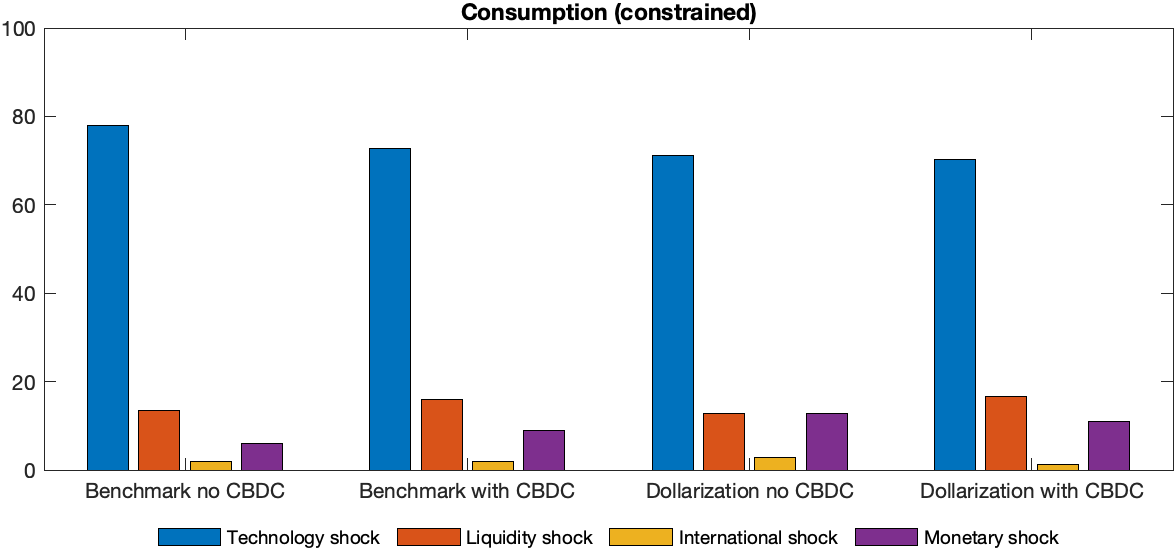
\includegraphics[width=0.8\textwidth]{log_c2}
\caption{Variance decomposition of consumption (constrained)}
\label{log_c2}
\end{figure}

Figure \ref{log_c2} shows the variance decomposition of consumption for the constrained households. Both introduction of CBDC and the dollar decrease the effect of TFP on the volatility of the consumption of constrained households. Dollarization increases the exposure of constrained households to international shocks, while CBDC decreases it. The adoption of CBDC decreases the volatility attributable to policy shocks. 

\begin{figure}[h!]
\centering
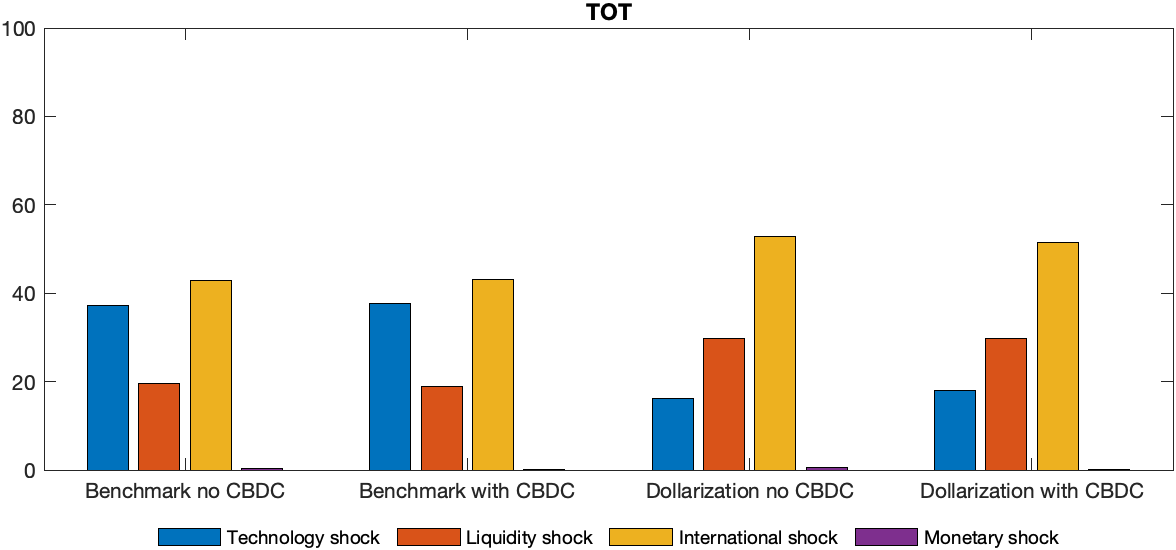
\includegraphics[width=0.8\textwidth]{log_tot}
\caption{Variance decomposition of terms of trade}
\label{log_tot}
\end{figure}

Figure \ref{log_tot} shows the variance decomposition of terms of trade. Dollarization amplifies the effect of international shocks on the terms of trade. Adoption of CBDC decreases the responses of terms of trade to international shocks. 

\section{Impulse Response}

\begin{figure}[h!]
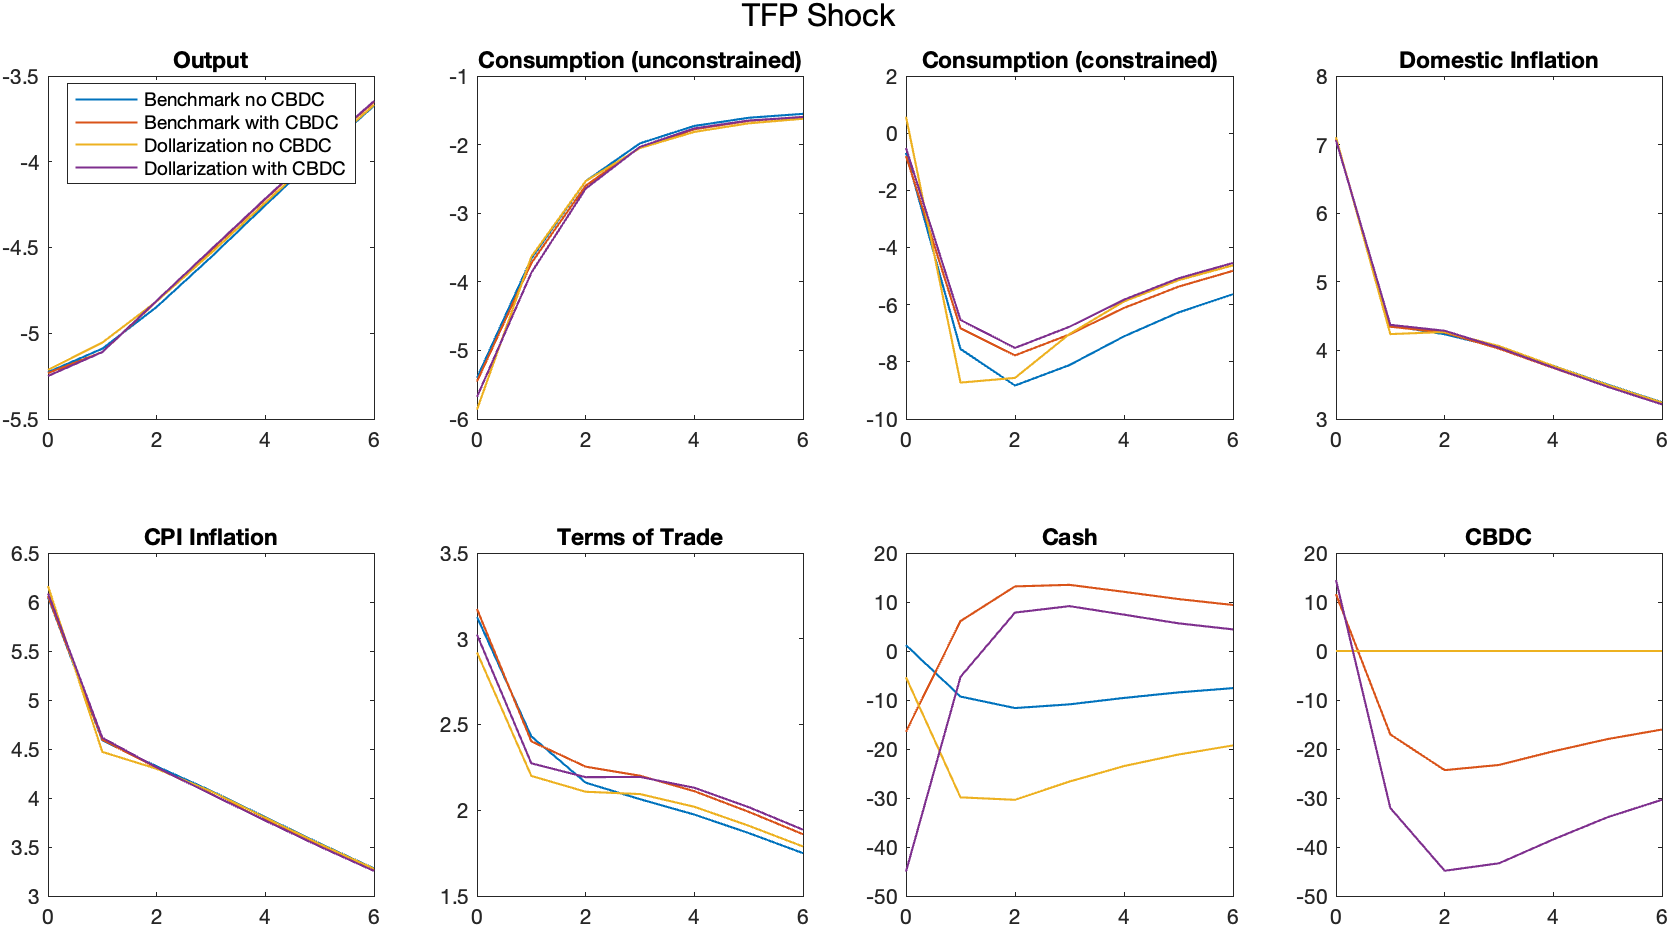
\includegraphics[width=\textwidth]{TFP}
\caption{Impulse Responses of TFP Shock}
\label{IRF1}
\scriptsize{Notes: Response of key variables to a negative 1 standard deviation TFP shock. The Vertical axis indicates the percentage deviation from the steady state. The horizontal axis indicates years after the shock. }
\end{figure}
Figure \ref{IRF1} plots the responses of key variables following a negative TFP shock. The introduction of CBDC decreases the responses of consumption to TFP shocks. CBDC promotes the financial inclusion of constrained households and decreases the volatility of consumption. The constrained households switch more to CBDC following a negative TFP shock since they are more sensitive to the cost of cash and rely more on CBDC to smooth out their consumption. The terms of trade respond less to TFP shocks when CBDC is introduced as a result of the portfolio adjustment. 

\begin{figure}[h!]
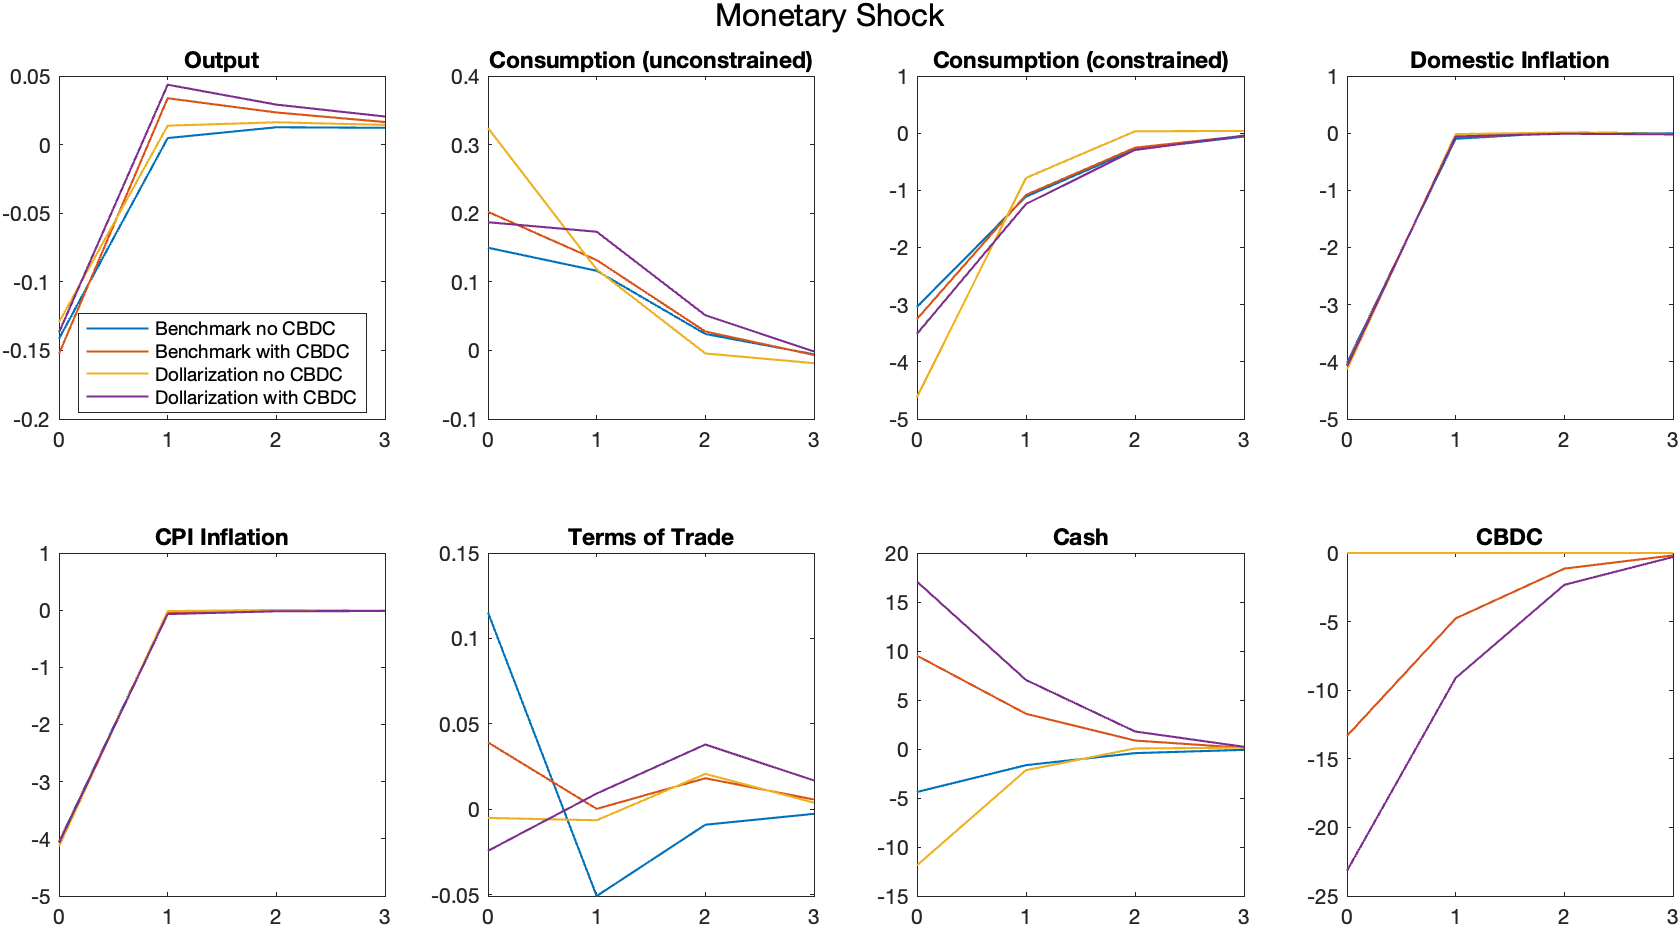
\includegraphics[width=\textwidth]{Monetary}
\caption{Impulse Responses of Monetary Policy Shock}
\label{IRF2}
\scriptsize{Notes: Response of key variables to a positive 1 standard deviation monetary policy shock. The Vertical axis indicates the percentage deviation from the steady state. The horizontal axis indicates years after the shock. }
\end{figure}
Figure \ref{IRF2} plots the responses of key variables following a positive monetary shock. A positive monetary policy shock favors unconstrained households since they receive a higher payoff to their deposit. The introduction of CBDC decreases the inequality effect of monetary policy. 

\begin{figure}[h!]
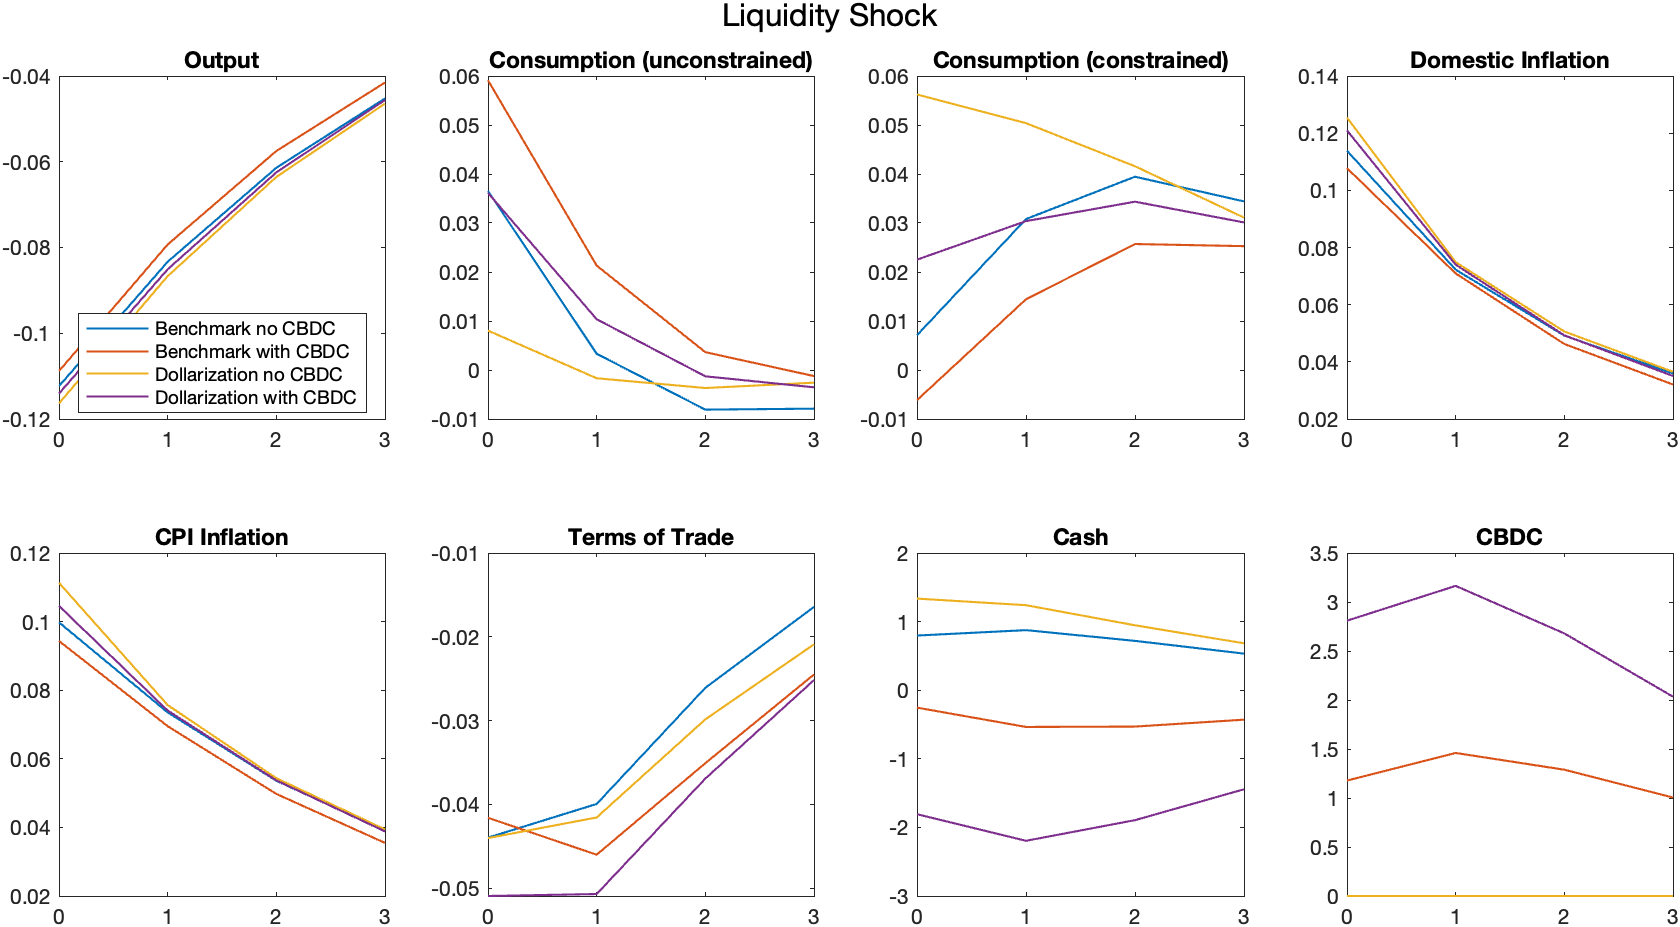
\includegraphics[width=\textwidth]{Liquidity}
\label{IRF3}
\caption{Impulse Responses of Liquidity Shock}
\scriptsize{Notes: Response of key variables to a positive 1 standard deviation liquidity shock. The Vertical axis indicates the percentage deviation from the steady state. The horizontal axis indicates years after the shock.}
\end{figure}

\begin{figure}[h!]
\includegraphics[width=\textwidth]{Y_STAR}
\label{IRF4}
\caption{Impulse Responses of Foreign Output Shock}
\scriptsize{Notes: Response of key variables to a positive 1 standard deviation foreign output shock. The Vertical axis indicates the percentage deviation from the steady state. The horizontal axis indicates years after the shock.}
\end{figure}

\begin{figure}[h!]
\includegraphics[width=\textwidth]{R_STAR}
\label{IRF5}
\caption{Impulse Responses of Foreign Interest Rate Shock}
\scriptsize{Notes: Response of key variables to a positive 1 standard deviation foreign interest rate shock. The Vertical axis indicates the percentage deviation from the steady state. The horizontal axis indicates years after the shock.}
\end{figure}


\end{document}